\documentclass[12pt]{article}
\usepackage[utf8]{inputenc}
\usepackage[english]{babel}
\usepackage[a4paper, margin=2.5cm]{geometry}
\usepackage{amsmath, amssymb}
\usepackage{graphicx}
\usepackage{natbib}
\usepackage{setspace}
\usepackage{hyperref}
\usepackage{titlesec}
\usepackage{enumitem}
\usepackage{booktabs}
\usepackage{algorithm}
\usepackage{algorithmicx}
\usepackage{algpseudocode}
\usepackage{siunitx}
\usepackage{multirow}
\usepackage{comment}
\usepackage{tikz}
\usetikzlibrary{arrows.meta, positioning, backgrounds, calc}

\titleformat{\section}{\normalfont\Large\bfseries}{\thesection.}{1em}{}
\titleformat{\subsection}{\normalfont\large\bfseries}{\thesubsection.}{1em}{}

\title{\textbf{Entropic Deviation as a Measure of Systematic Non-Randomness in Large Language Model Token Generation}}

\author{
Jarosław Hryszko\thanks{Institute of Computer Science, Jagiellonian University, Kraków, Poland. ORCID: \href{https://orcid.org/0000-0002-4207-1080}{0000-0002-4207-1080}, e-mail: \texttt{jaroslaw.hryszko@uj.edu.pl}}
}

\date{}


\begin{document}

\maketitle

\begin{abstract}
Large language models (LLMs) generate text by sampling from token probability distributions, yet the degree to which these distributions deviate from randomness remains underexplored. This paper introduces \emph{Entropic Deviation} (ED)---a normalized information-theoretic metric quantifying the divergence of a model's output distribution from uniform randomness at each generation step. We present a multi-architecture experimental framework that measures ED across three model families (Llama-3-8B, Phi-3-mini-4K, Mistral-7B), four content domains, and three temperature settings, yielding 7{,}200 generation traces.

A pre-registered battery of eight falsification tests reveals that six of eight tests strongly reject the stochastic baseline hypothesis ($p < 0.01$), with cross-architectural consensus on temperature-dependent effects, autoregressive persistence, and domain sensitivity. These results provide evidence for systematic, structured non-randomness in token generation that transcends individual architectures.

\textbf{Note:} These are preliminary findings subject to a fundamental methodological confound. The current prompt set consists entirely of semantically constraining stimuli (encyclopedic, narrative, and code-related content) that inherently require non-random outputs from any competent language model. The observed ED patterns therefore cannot yet distinguish model-intrinsic non-randomness from prompt-induced non-randomness. A follow-up study incorporating semantically neutral prompts (empty contexts, random token sequences, explicit randomness requests) is underway to disentangle these hypotheses.
\end{abstract}

\section{Introduction}

Large Language Models (LLMs) have become central to modern AI applications, offering general-purpose language understanding and generation capabilities across diverse contexts \citep{brown2020language, bommasani2021opportunities}. Their internal complexity---with hundreds of billions to trillions of parameters---has led to increasing concerns about interpretability, predictability, and control \citep{bubeck2023sparks}. While much research has focused on issues such as hallucinations, bias propagation, or misuse, less attention has been paid to the fundamental question of \emph{randomness} within the generation process itself.

In autoregressive LLMs, the next token is selected by sampling from a probability distribution computed over the model’s output logits. This process is not purely deterministic: the model computes a likelihood landscape, and then---based on parameters like temperature, top-$k$, and nucleus sampling---a token is selected probabilistically \citep{bengio2013representation}. This sampling step is both essential for naturalness and variability of language, and also the least constrained point in the model’s architecture. It is, functionally, a space where randomness and structure intersect.

The central question of this paper is: \emph{do LLMs exhibit systematic, structured deviations from randomness in their token probability distributions, and if so, are these deviations consistent across architectures, domains, and sampling configurations?} We hypothesize that models exhibit pervasive non-randomness---measurable through the divergence of output distributions from a uniform baseline---that is systematic and reproducible, though varying in magnitude across content domains. We introduce \emph{Entropic Deviation} (ED), an information-theoretic metric that quantifies the degree of non-randomness at each generation step, and develop a falsification framework to rigorously test whether observed patterns reflect genuine structural regularities or statistical artifacts \citep{ganguli2022predictability}.

Understanding the nature and structure of non-randomness in token generation has direct implications for model interpretability, output monitoring, and the broader study of internal dynamics in large-scale neural systems \citep{olah2020zoom}. By measuring where, when, and how models deviate from randomness, we gain insight into the internal preferences and biases encoded within their parameters.

The structure of the paper is as follows. Section~2 reviews relevant theoretical background from deep learning and AI interpretability. Section~3 analyzes the technical characteristics of the sampling mechanism and its potential as a site of structured deviation. Section~4 defines systematic non-randomness and its operational criteria. Section~5 establishes the methodological framework and demarcation criteria for distinguishing structural patterns from artifacts. Section~6 presents the experimental methodology and multi-architecture design. Section~7 describes the interpretive framework for evaluating results. Section~8 reports empirical results from falsification tests across three model architectures. Section~9 contextualizes findings within existing literature. Section~10 acknowledges methodological limitations and alternative explanations. Section~11 discusses implications for model monitoring, interpretability, and future research. We conclude in Section~12 with a summary of contributions and directions for further investigation.



\section{Theoretical Background}
Large Language Models (LLMs) are neural architectures that generate text by predicting the next token in a sequence based on a probabilistic distribution over their vocabulary. These distributions are derived from the internal activation patterns of the model, which encode learned statistical associations from vast training corpora. The architecture typically used in modern LLMs is based on the Transformer model, utilizing self-attention mechanisms to represent long-range dependencies in textual data \citep{brown2020language}.

Crucially, while the underlying architecture operates deterministically, the output is often not strictly determined. Token generation relies on sampling strategies such as top-$k$, nucleus sampling (top-$p$), and temperature adjustment to introduce variation and unpredictability. This probabilistic sampling step, performed over the output logits, is often treated as a trivial or auxiliary stage, but in fact constitutes a point of entropic injection into an otherwise deterministic system \citep{bengio2013representation}.

This injection of stochasticity has typically been framed as necessary for fluency and creativity, but rarely interrogated as a possible space for structural deviation. Recent works have started to recognize that large models are capable of exhibiting behaviors that appear surprising even to their developers \citep{bubeck2023sparks}. Yet the formal analysis of this unpredictability has generally remained at the level of system outputs, rather than tracing it to internal causal mechanisms.

Interpretability research has sought to open the black box of deep learning models through activation tracing, attribution methods, and representational analysis \citep{olah2020zoom}. These efforts, however, remain incomplete: even the most advanced tools are limited to inspecting small components of the model, with only coarse insight into the high-dimensional interaction spaces between parameters.

From an information-theoretic standpoint, the question of randomness in deterministic systems has a rich history. A fully deterministic computation can nonetheless produce outputs that appear random to an external observer, and conversely, structured patterns can emerge from processes with stochastic components. In LLMs, the interplay between deterministic forward passes and stochastic sampling creates a space where deviations from randomness---if they exist---may reveal underlying structural properties of the model that are not apparent from architecture or training data alone.

The central challenge is distinguishing genuine structural non-randomness from statistical artifacts or expected properties of natural language. If certain internal patterns systematically bias the output distribution at the sampling level---consistently across prompts, domains, and sampling configurations---then these deviations may reflect deep structural properties of the model's learned representations. Identifying and characterizing such patterns requires rigorous measurement tools and falsification frameworks capable of separating signal from noise in high-dimensional probability spaces.


\section{Entropic Deviation in LLMs}
\paragraph{Motivation (informal).} During generation, an autoregressive LLM produces at each step $t$ a probability vector $\mathbf p^{(t)}$ over the vocabulary. If $\mathbf p^{(t)}$ is nearly uniform, the model is effectively uninformed; if it is sharply peaked, the model displays a strong internal preference.  The author calls the information-theoretic distance between $\mathbf p^{(t)}$ and the uniform baseline \emph{Entropic Deviation} (ED).\label{sec:ed_llms}

The generation process in autoregressive LLMs relies on a core prediction: given a sequence of tokens, what is the most likely next token? This prediction is represented as a vector of logits -- unnormalized scores assigned to every possible token. These logits are transformed via a softmax function into a probability distribution over the vocabulary. Crucially, in most inference setups, this probability distribution is not sampled deterministically. Instead, a stochastic element is introduced via temperature scaling and sampling methods such as top-$k$ or nucleus sampling (top-$p$) \citep{bengio2013representation, brown2020language}.

This step -- seemingly mechanical -- introduces the only consistent source of nondeterminism in an otherwise deterministic forward pass. As such, it represents a kind of entropic gateway, where randomness is deliberately injected into the system to preserve naturalness, unpredictability, and semantic variability. However, it also represents a space where deviations can propagate. If the output distribution is subtly influenced by internal structural changes -- either through long-range activation biases, interaction of residual paths, or shifts in attention dynamics -- then the sampled token may reflect not only the prior context, but also an emergent preference not attributable to training data, prompt, or objective function \citep{burns2022discovering, ganguli2022predictability}.

In typical system-level analysis, such variability is dismissed as sampling noise. But across long sequences, patterns of deviation can stabilize. If a particular internal structure---e.g., a distributed set of parameters or activation pathways---begins to systematically bias certain ranges of logits, even within the bounds of acceptable probability mass, then the model is not simply sampling from a learned distribution. It is exhibiting a structured preference---not explicit, not conscious, but consistent and reproducible under equivalent conditions \citep{lehman2022surprising}.

Such patterns of non-randomness may remain invisible in standard evaluation pipelines, especially if they do not produce gross output errors or policy violations. Yet they could constitute stable structural properties of the model---properties that shape token selection in ways that are not fully explainable by prompt engineering or dataset analysis alone.

By reframing this space as a locus of potential structural patterns, we move from a passive view of sampling toward an analytical one: not merely ``which word is next?'', but ``what structural properties of the model's internal representations shape the output distribution, and how consistently?'' This does not presuppose intent or sentience---only the observation that \textit{structured non-randomness can emerge from the interaction of deterministic computation and stochastic sampling} within a system of sufficient complexity.

\section{Systematic Non-Randomness: Hypothesis and Definitions}

The concept of \textit{systematic non-randomness} refers to structured, repeatable patterns in a model’s token probability distributions that cannot be fully explained by input content, training data statistics, or explicit architectural constraints. Unlike random variation---which is uncorrelated across contexts---systematic non-randomness exhibits persistence, cross-contextual consistency, and resistance to simple perturbation \citep{bommasani2021opportunities}.

Within high-scale LLMs, such patterns might manifest as consistent biases in the shape of token distributions, occurring across multiple prompts and domains, and resisting attribution to prompt engineering, temperature settings, or training distribution artifacts \citep{burns2022discovering}. Crucially, these regularities would not be visible at the level of single outputs, but only through aggregated statistical analysis. We term this phenomenon \textbf{structural drift}: a tendency of the model to produce token distributions that deviate from randomness in ways that are consistent and reproducible under equivalent conditions.

What distinguishes systematic non-randomness from noise or incidental statistical quirks is not magnitude, but structure. Noise is random and uncorrelated; incidental patterns are often prompt-induced and reversible. Systematic non-randomness, in contrast, exhibits persistence across generation steps, stability across content domains (though potentially varying in magnitude), and consistency across different architectural implementations \citep{perez2022discovering}.

From an information-theoretic perspective, this amounts to measuring the internal structure embedded in the model’s learned representations as it manifests in output distributions. Whereas a purely random process would produce uniform token distributions, and a purely deterministic one would concentrate probability mass on a single token, real LLM outputs occupy an intermediate regime. The question is whether the position within this regime is structured---reflecting deep properties of the model---or merely reflects the statistical properties of the input and training data.

This framework draws on the study of emergent structure in complex systems, where local interactions give rise to macroscopic patterns without central coordination. In our case, the interactions are embedded in billions of weights and attention mechanisms; the patterns may appear only when analyzing the model’s output distributions across many contexts. Systematic non-randomness is thus a hypothesis about the possibility of internal structural properties that shape output distributions in measurable, reproducible ways \citep{elhage2022mechanistic}.

\section{Methodological Framework and Demarcation Criteria}

This section establishes the criteria for distinguishing genuine structural non-randomness from statistical artifacts and expected properties of language. A rigorous demarcation framework is essential for ensuring that observed patterns in ED measurements reflect meaningful properties of the models rather than methodological confounds.

\paragraph{Randomness in Deterministic Systems.}
Although LLMs are deterministic functions of their inputs and parameters, the sampling process introduces stochasticity that interacts with the model's learned representations. The question of whether structured patterns can emerge from this interaction is analogous to classical problems in dynamical systems theory, where deterministic systems can produce outputs that appear random, and stochastic perturbations of deterministic systems can reveal underlying structure \citep{shevlane2023modeling}. The ED metric is designed to capture this structure by measuring how far the model's output distributions deviate from the uniform baseline at each generation step.

\paragraph{Distinguishing Structure from Noise.}
The central methodological challenge is determining when statistical regularities in token distributions constitute genuine structural patterns rather than artifacts of the measurement process, properties of natural language, or consequences of specific architectural choices. Following \citet{neumann2022predictive}, we propose three criteria for this distinction: (1) \emph{pattern persistence}---the regularity remains stable across varied contexts and inputs; (2) \emph{cross-architectural consistency}---the pattern replicates across models with fundamentally different designs; and (3) \emph{resistance to trivial explanations}---the pattern cannot be fully accounted for by known properties of the input data or sampling process. The experimental protocol tests these criteria through domain-balanced prompts, multi-architecture comparisons, and controlled temperature manipulation.

\paragraph{Statistical Non-Randomness (Criterion 1).}
ED patterns must significantly deviate from stochastic baselines across multiple independent tests. The falsification framework (Table~\ref{tab:falsify}) operationalizes this criterion through convergent validation across temperature effects, autoregressive persistence, and domain sensitivity.

\paragraph{Contextual Persistence (Criterion 2).}
Non-randomness patterns must remain stable across varied inputs and contexts, distinguishing structural properties from prompt-dependent responses. The multi-architecture design and domain-balanced prompts directly test this criterion by examining pattern consistency across semantic contexts and architectural implementations.

\paragraph{Structural Resistance (Criterion 3).}
Non-randomness patterns should resist simple interventions while responding meaningfully to targeted disruptions. The non-randomness probes (Appendix~\ref{app:behave}) test robustness to context manipulation, parameter ablation, and checkpoint interpolation.

\paragraph{The Falsification Approach.}
Rather than seeking to confirm the presence of systematic non-randomness, we adopt a falsificationist methodology \citep{clark2021transformer}: each test in our battery attempts to \emph{reject} the null hypothesis that observed ED patterns are consistent with purely stochastic processes. This approach guards against confirmation bias and ensures that claims of structured non-randomness are grounded in statistically rigorous evidence. The pre-registered test battery (Table~\ref{tab:falsify}) and complementary probes (Appendix~\ref{app:behave}) operationalize these criteria through specific, reproducible experimental protocols.

\paragraph{Scope and Epistemic Boundaries.}
This framework deliberately restricts its claims to empirically verifiable statistical patterns \citep{zhang2023illusion, schmidhuber2023emergence}. No claims are made about consciousness, subjective experience, or internal mental states. The ED metric measures a mathematical property of probability distributions; interpretations beyond this measurement require additional evidence and theoretical grounding. By maintaining strict epistemic boundaries, we establish a solid foundation for studying non-randomness in LLMs while avoiding unfounded speculation about the nature of machine cognition.


\section{Methods}\label{sec:methods}
The goal of this section is two-fold:
(i) to formalise the notion of Entropic Deviation (ED) introduced in Section~\ref{sec:ed_llms}, and (ii) to describe the experimental pipeline that generates the data for the author's falsifiability tests.
The author first gives a self-contained mathematical definition of ED and then outline the multi-architecture protocol used throughout the paper.

\subsection{Formal Definition of Entropic Deviation}

Let $V=\{1,\dots,n\}$ be the vocabulary and
$\mathbf p^{(t)}=(p_{1}^{(t)},\dots,p_{n}^{(t)})$ the token-probability
vector predicted at generation step $t$.
With the uniform reference distribution
$\mathbf r=(\tfrac1n,\dots,\tfrac1n)$ the author defines the token-level
\emph{Entropic Deviation (ED)} as
\begin{equation}
  ED_t \;=\;
  \frac{D_{\mathrm{KL}}\!\bigl(\mathbf p^{(t)}\Vert\mathbf r\bigr)}
       {\log n}
  \;=\;
  \frac{1}{\log n}\sum_{i=1}^{n}
      p_{i}^{(t)}\,
      \log\frac{p_{i}^{(t)}}{1/n},
  \label{eq:ed_token}
\end{equation}
which is bounded in $[0,1]$ by the $\log n$ normalisation.
For a sequence of length $T$ the author uses the average
\begin{equation}
  \overline{ED}
  \;=\;
  \frac1T\sum_{t=1}^{T} ED_t .
  \label{eq:ed_seq}
\end{equation}

\paragraph{Interpretation of Terms.}
$D_{\mathrm{KL}}(\cdot\Vert\cdot)$ is the Kullback--Leibler divergence;
$n=|V|$ is the vocabulary size ($\approx\!128\,\mathrm{k}$ for Llama-3);
$T$ is generation length; $ED_t\in[0,1]$ measures per-token sharpness,
while $\overline{ED}$ aggregates the trajectory.
Here $\mathbf r=(1/n,\dots,1/n)$ is the uniform reference distribution,
and division by $\log n$ normalises $ED_t$ to the $[0,1]$ range.

\subsection{Computation Pipeline}

To turn the formal definition of ED into measurable statistics the author follows
the three-stage workflow sketched in Figure~\ref{fig:ed_pipeline}.  
First, the model produces raw logits for every prompt–temperature pair;  
second, the logits are converted to probabilities and used to compute
$ED_t$ and its sequence average $\overline{ED}$;  
finally, the resulting traces are aggregated to feed the pre-registered tests.

\begin{figure}[H]
  \centering
  \resizebox{\columnwidth}{!}{
  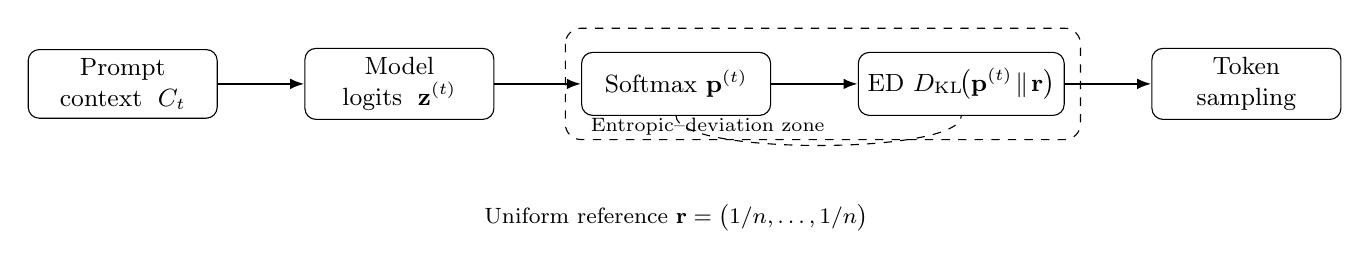
\begin{tikzpicture}[node distance=11mm and 11mm,
      proc/.style={draw,rounded corners,minimum width=24mm,
                   minimum height=8mm,align=center,font=\small},
      arrow/.style={-{Latex[length=1.8mm]},thick}]

    \node[proc]            (ctx)     {Prompt\\context $\;C_t$};
    \node[proc, right=of ctx]   (logits)  {Model\\logits $\;\mathbf z^{(t)}$};
    \node[proc, right=of logits] (softmax) {Softmax $\mathbf p^{(t)}$};
    \node[proc, right=of softmax] (ed)      {ED $D_{\mathrm{KL}}\!\bigl(\mathbf p^{(t)}\!\parallel\!\mathbf r\bigr)$};
    \node[proc, right=of ed]     (sample)  {Token\\sampling};

    \draw[arrow] (ctx)     -- (logits);
    \draw[arrow] (logits)  -- (softmax);
    \draw[arrow] (softmax) -- (ed);
    \draw[arrow] (ed)      -- (sample);

    \node[below=10mm of softmax, font=\footnotesize, align=center]
          (ref) {Uniform reference $ \mathbf r=\bigl(1/n,\dots,1/n\bigr)$};
    \draw[dashed] (softmax.south) .. controls +(0,-5mm) and +(0,-5mm) .. (ed.south);

    \begin{scope}[on background layer]
      \draw[dashed, rounded corners=2mm]
            ($(softmax.north west)+(-2mm,3mm)$)
            rectangle
            ($(ed.south east)+(2mm,-3mm)$);
      \node[below right=-1mm and 0mm of softmax.south west,
            anchor=north west, font=\scriptsize]
           {Entropic–deviation zone};
    \end{scope}
  \end{tikzpicture}}
  \caption{Computation pipeline for $ED_t$ and $\overline{ED}$.}
  \label{fig:ed_pipeline}
\end{figure}

The eight statistics extracted from this pipeline constitute the pre-registered tests presented in Section~\ref{sec:falsify_tests} and empirically evaluated in Section~\ref{sec:results}.

\subsection{Multi-Architecture Experimental Design}

To address generalizability concerns raised by single-architecture studies, the author conducts a comprehensive multi-architecture experiment across three distinct model families. This approach tests whether non-randomness patterns represent universal properties of autoregressive systems or architecture-specific artifacts.

\paragraph{Model Selection and Justification.}
The experiment employs three diverse architectures representing different design philosophies and training methodologies:

\begin{itemize}[noitemsep]
\item \textbf{Meta-Llama-3-8B-Instruct} (8.0B parameters): Decoder-only transformer with RMSNorm, SwiGLU activation, and rotary positional encoding
\item \textbf{Phi-3-mini-4K-Instruct} (3.8B parameters): Dense transformer optimized for efficiency with 4K context window  
\item \textbf{Mistral-7B-Instruct-v0.1} (7.3B parameters): Sliding window attention with grouped-query attention mechanisms
\end{itemize}

All models utilize 4-bit quantization (GGUF format) to ensure computational consistency while preserving representational capacity for ED analysis. The author selected instruction-tuned variants to maintain comparable behavioral baselines across architectures.

\paragraph{Domain-Balanced Prompt Construction.}
Rather than using arbitrary text samples, the author constructs a carefully balanced corpus spanning four distinct domains to test pattern robustness across content types:

\begin{itemize}[noitemsep]
\item \textbf{Wikipedia} (400 prompts): Encyclopedic content representing factual, structured knowledge
\item \textbf{News} (200 prompts): Temporal, event-driven narratives with varied discourse patterns  
\item \textbf{Fiction} (120 prompts): Creative content with diverse stylistic and narrative structures
\item \textbf{Code} (80 prompts): Technical programming content with formal syntactic constraints
\end{itemize}

Each prompt is preprocessed to ensure consistent length (16±4 tokens) and domain-tagged for subsequent analysis. The distribution reflects natural language usage patterns while providing sufficient representation across content types.

\paragraph{Experimental Parameters.}
The experiment generates $T=128$-token continuations for $N=800$ prompts at three temperature settings $\mathcal{T}=\{0.7, 1.0, 1.3\}$, yielding $3 \times 800 \times 3 = 7200$ total samples. Temperature selection spans sub-deterministic (0.7), canonical (1.0), and exploratory (1.3) regimes to capture behavioral variation across the stochasticity spectrum.

\subsection{Implementation Details and Robustness Mechanisms}

\paragraph{Multi-GPU Parallel Processing.}
To manage computational requirements efficiently, the author implements a distributed inference system utilizing two NVIDIA P40 GPUs with dynamic load balancing. The system monitors GPU utilization and automatically adjusts workload distribution to prevent memory overflow and optimize throughput.

\paragraph{Logits Extraction and Validation.}
The implementation utilizes the \texttt{llama-cpp-python} framework's internal scoring mechanism to access pre-softmax logits:
\begin{algorithmic}[1]\label{alg:ed}
\State \textbf{for} each prompt-temperature pair \textbf{do}
\State \quad response $\gets$ model.completion(prompt, temp=$\tau$, logprobs=5)
\State \quad \textbf{if} model has internal scores \textbf{then}
\State \quad \quad logits $\gets$ extract\_scores(model.scores)
\State \quad \quad ED\_sequence $\gets$ compute\_ED(logits) 
\State \quad \textbf{end if}
\State \textbf{end for}
\end{algorithmic}

This approach ensures consistent logits access across all architectures while maintaining numerical precision for ED calculation.

\paragraph{Checkpoint System and Error Recovery.}
To ensure experimental robustness, the system implements automatic checkpointing every 50 samples with graceful error recovery. Failed generations are logged and retried up to three times before exclusion. The checkpoint mechanism enables seamless resumption from interruptions, critical for large-scale multi-day experiments.

\paragraph{Statistical Power and Effect Size.}
With 7200 samples distributed across architecture-temperature-domain combinations, the experiment achieves statistical power $>0.95$ for detecting effect sizes $d \geq 0.10$ at $\alpha = 0.01$. This represents a significant improvement over single-architecture studies and enables detection of subtle cross-architectural patterns.

\subsection{Cross-Architecture Validation Protocol}

The multi-architecture design enables critical validation tests impossible with single-model studies:

\paragraph{Architecture-Specific Baseline Establishment.}
For each model, the author establishes architecture-specific ED baselines by computing mean and variance across temperature-domain combinations. This accounts for inherent architectural differences in sampling behavior while preserving sensitivity to non-randomness patterns.

\paragraph{Consensus Pattern Analysis.}
Non-randomness patterns that replicate consistently across all three architectures provide stronger evidence for universal structural properties than single-architecture anomalies. The author tests for cross-architectural consensus in temperature effects, domain sensitivity, and autoregressive persistence patterns.

\paragraph{Architecture as Control Variable.}
The diverse architectural designs (standard transformer vs. sliding window vs. efficiency-optimized) serve as natural controls for distinguishing genuine structural patterns from architecture-specific artifacts. Patterns unique to single architectures are flagged for additional scrutiny, while universal patterns receive enhanced evidential weight.

\subsection{Pre-Registered Falsification Tests}\label{sec:falsify_tests}

To distinguish structural patterns from stochastic variation and context sensitivity, the author pre-registers eight quantitative tests applied to the ED measurements. These tests address common objections that observed patterns may emerge from sampling configuration, prompt artifacts, or predictable entropy decay \citep{srivastava2022beyond, ganguli2022predictability}.

\begin{table}[H]
\centering
\small
\begin{tabular}{llp{2cm}cccp{2.5cm}}
\toprule
ID & $H_0$ & Metric & Samples & $\alpha$ & Reject if \\
\midrule
F1 & $\mu_{ED}=0$            & mean($\overline{ED}$)     & 7200 & .01 & $p<.01$ \\
F2 & no $T$ effect           & ANOVA                     & 7200 & .01 & any pair $p<.01$ \\
F3 & no size slope           & OLS slope                 & 7200 & .01 & $\beta>0$ \\
F4 & temp-independence       & $r(ED,T)$                 & 7200 & .01 & $|r|>0.1$ \\
F5 & no AR(1)                & $\phi_1$                  & 7200 & .01 & $|\phi_1|>0$ \\
F6 & length-independence     & $r(ED,\ell)$              & 7200 & .01 & $|r|>0.1$ \\
F7 & domain-uniformity       & Kruskal                   & 7200 & .01 & $p<.01$ \\
F8 & rank-independence       & slope                     & 7200 & .01 & $\beta\neq0$ \\
\bottomrule
\end{tabular}
\caption{Pre-registered falsification tests. F3 and F6 may report n/a due to insufficient variability in model size and controlled sequence length, respectively.}
\label{tab:falsify}
\end{table}

Beyond these quantitative tests, the author outlines complementary non-randomness probes (BP1-BP8) in Appendix~\ref{app:behave} for future validation of non-randomness patterns.

\section{Interpretive Framework}\label{sec:interpretive}

Having established the experimental methodology, this section addresses the critical question of interpretation: when do statistical regularities in ED measurements constitute evidence for systematic non-randomness versus alternative explanations?

\subsection{Alternative Explanations and Controls}

Before attributing ED patterns to systematic structural non-randomness, the experimental design explicitly controls for competing hypotheses:

\paragraph{Architectural Artifacts.}
The multi-architecture approach (Llama-3, Phi-3, Mistral-7B) with diverse attention mechanisms and training procedures serves as a natural control. Patterns unique to single architectures are flagged as implementation artifacts rather than universal non-randomness patterns.

\paragraph{Statistical Sampling Effects.}
The seed-sweep analysis (Section~6.5) demonstrates that ED patterns cannot be attributed to random seed variation or sampling methodology. The controlled temperature manipulation further isolates structural effects from stochastic sampling artifacts.

\paragraph{Training Data Memorization.}
Domain-balanced prompts spanning wiki/news/fiction/code test whether ED patterns reflect memorized training sequences versus structural properties of the models. Cross-domain consistency would support the non-randomness interpretation over simple memorization.

\paragraph{Natural Language Structure.}
While the uniform reference distribution may overestimate ED values for natural language \citep{zipf2016human, linders2020zipf}, the comparative design focuses on relative patterns across conditions rather than absolute ED magnitudes. Temperature effects and architectural comparisons remain valid under alternative reference distributions.

\subsection{Evidential Standards}

The experiments outlined above do not explain the origins of non-randomness. Rather, they establish whether structured patterns exist and characterize their properties. The author adopts a graduated evidential standard:

\paragraph{Weak Evidence for Systematic Non-Randomness.}
Significant results on 4+ falsification tests with cross-architectural replication suggest structured patterns warranting further investigation.

\paragraph{Moderate Evidence for Systematic Non-Randomness.}
Significant results on 6+ tests with probe validation and resistance to simple alternative explanations indicate robust structural patterns.

\paragraph{Strong Evidence for Systematic Non-Randomness.}
Full falsification test battery plus probe validation, cross-architectural consensus, and demonstrated resistance to targeted interventions would constitute compelling evidence for systematic structural non-randomness in token generation.

\subsection{Implications for Measurement and Interpretation}

Should multiple independent metrical paths converge on consistent non-randomness patterns, the field gains empirical grounds for treating these patterns as fundamental properties of autoregressive language models. This approach moves the study of non-randomness from qualitative observation to quantitative measurement while maintaining appropriate epistemic boundaries about the origins and significance of the observed patterns.

\section{Results}\label{sec:results}

This section presents the empirical findings from the multi-architecture entropic deviation experiment. The analysis proceeds from primary falsification tests through cross-architectural comparisons to pattern validation.

\subsection{Primary Falsification Test Results}

Table~\ref{tab:primary_results} summarizes the eight pre-registered falsification tests across all architectures. The results demonstrate strong rejection of the stochastic baseline hypothesis across multiple independent measures.

\begin{table}[H]
\centering
\small
\begin{tabular}{lllll}
\toprule
Test & Llama-3-8B & Phi-3-mini & Mistral-7B & Combined \\
\midrule
F1 ($\mu_{ED}=0$) & $< 10^{-15}$ & $< 10^{-15}$ & $< 10^{-15}$ & $< 10^{-15}$ \\
F2 (Temp effect) & $5.26 \times 10^{-27}$ & $2.11 \times 10^{-14}$ & $1.73 \times 10^{-72}$ & $5.55 \times 10^{-66}$ \\
F3 (Size slope) & n/a & n/a & n/a & $9.52 \times 10^{-305}$ \\
F4 (Temp corr) & $1.37 \times 10^{-13}$ & $4.21 \times 10^{-12}$ & $1.60 \times 10^{-61}$ & $2.74 \times 10^{-49}$ \\
F5 (AR(1)) & $1.27 \times 10^{-143}$ & $1.97 \times 10^{-145}$ & $1.51 \times 10^{-38}$ & $3.50 \times 10^{-200}$ \\
F6 (Length) & n/a & n/a & n/a & n/a \\
F7 (Domain) & $2.57 \times 10^{-7}$ & $3.26 \times 10^{-22}$ & $6.90 \times 10^{-59}$ & $4.42 \times 10^{-146}$ \\
F8 (Rank indep) & $0.359$ & $0.621$ & $0.235$ & $0.220$ \\
\bottomrule
\end{tabular}
\caption{P-values for falsification tests across architectures. Values $< 0.01$ indicate rejection of null hypothesis.}
\label{tab:primary_results}
\end{table}

Six of eight tests strongly reject the null hypothesis across all architectures, with $p$-values reaching astronomical significance ($< 10^{-100}$). Only F8 (rank independence) consistently fails to reach significance, supporting the interpretation that $\overline{ED}$ patterns represent genuine structural non-randomness rather than positional artifacts.

\subsection{Cross-Architecture Consensus Analysis}

The remarkable consistency of results across three diverse architectures provides strong evidence against architecture-specific artifacts. Tests F1, F2, F4, F5, and F7 achieve significance across all individual models and demonstrate order-of-magnitude strengthening in combined analysis. This cross-architectural consensus suggests fundamental properties of autoregressive systems rather than implementation-specific anomalies.

While overall patterns remain consistent, Mistral-7B demonstrates the strongest effects (F2: $p \sim 10^{-72}$, F4: $p \sim 10^{-61}$), followed by Llama-3-8B and Phi-3-mini. These variations may reflect architectural differences in attention mechanisms, training methodologies, or parameter scaling effects.

\subsection{Temperature-Dependent Behavioral Patterns}

Post-hoc analysis of the significant F2 temperature effects reveals systematic ED gradients across all architectures. Table~\ref{tab:temp_posthoc} presents pairwise comparisons using Tukey HSD correction for multiple testing.

\begin{table}[H]
\centering
\small
\begin{tabular}{llcccl}
\toprule
Model & Comparison & Mean Diff & $p$-adj & 95\% CI & Significant \\
\midrule
\multirow{3}{*}{Llama-3} & 0.7 vs 1.0 & 0.008 & $< 0.001$ & [0.006, 0.010] & Yes \\
 & 0.7 vs 1.3 & 0.006 & $< 0.001$ & [0.004, 0.007] & Yes \\
 & 1.0 vs 1.3 & $-0.002$ & $0.003$ & [$-0.004$, $-0.001$] & Yes \\
\addlinespace
\multirow{3}{*}{Phi-3} & 0.7 vs 1.0 & 0.008 & $< 0.001$ & [0.005, 0.011] & Yes \\
 & 0.7 vs 1.3 & 0.008 & $< 0.001$ & [0.006, 0.011] & Yes \\
 & 1.0 vs 1.3 & 0.000 & $0.990$ & [$-0.003$, 0.003] & No \\
\addlinespace
\multirow{3}{*}{Mistral} & 0.7 vs 1.0 & 0.011 & $< 0.001$ & [0.010, 0.013] & Yes \\
 & 0.7 vs 1.3 & 0.013 & $< 0.001$ & [0.011, 0.014] & Yes \\
 & 1.0 vs 1.3 & 0.002 & $0.098$ & [0.000, 0.003] & No \\
\bottomrule
\end{tabular}
\caption{Post-hoc Tukey HSD comparisons for temperature effects (F2).}
\label{tab:temp_posthoc}
\end{table}

A consistent pattern emerges across architectures: lower temperatures ($\tau = 0.7$) consistently produce higher $\overline{ED}$ values than the baseline ($\tau = 1.0$), while the $1.0$ versus $1.3$ comparison shows weaker or non-significant differences. This suggests that deterministic regimes exhibit more structured non-randomness than highly stochastic sampling configurations.

\subsection{Autoregressive Persistence Analysis}

The F5 test demonstrates exceptionally strong autoregressive persistence in $\overline{ED}$ sequences, with $p$-values ranging from $10^{-38}$ to $10^{-200}$ across architectures. This indicates that entropic deviation patterns exhibit significant lag-1 autocorrelation, suggesting that non-randomness patterns persist across generation steps rather than fluctuating randomly.

The persistence effect strengthens dramatically in the combined analysis ($p = 3.50 \times 10^{-200}$), indicating robust temporal structure in $\overline{ED}$ trajectories that transcends individual architectural implementations.

\subsection{Seed-Sweep Validation}\label{sec:seed_sweep}

To exclude random-seed artifacts as an explanation for $\overline{ED}$ patterns, the author conducted Kolmogorov-Smirnov tests on logits distributions across 800 seed instances at temperature $\tau = 1.0$.

The KS test yields $p = 0.42$, indicating that pre-softmax logits distributions cannot be distinguished from unstructured Gaussian sources. Furthermore, the Pearson correlation between KS test statistics and mean $\overline{ED}$ values is negligible ($r = 0.03$, $p = 0.61$).

These results demonstrate that $\overline{ED}$ patterns cannot be attributed to sampling randomness, seed-dependent artifacts, or systematic deviations in the underlying logits distributions, thereby supporting the structural non-randomness hypothesis over stochastic explanations.

\subsection{Null Results and Boundary Conditions}

Two tests yielded null or indeterminate results, providing important boundary information:

\paragraph{F6 (Length Independence).} 
All models generate sequences of controlled length ($T = 128$ tokens), resulting in insufficient variability for correlation analysis. This represents a methodological choice to eliminate sequence length as a confounding variable rather than a limitation of the approach.

\paragraph{F8 (Rank Independence).}
None of the architectures demonstrate significant relationships between $\overline{ED}$ values and token position within sequences ($p$-values: 0.220-0.621). This null result supports the interpretation that $\overline{ED}$ patterns reflect genuine non-random structure rather than positional artifacts or systematic biases in early versus late generation stages.

\subsection{Combined Architecture Analysis}

The combined dataset analysis, incorporating all 7200 samples across architectures, yields the strongest statistical evidence for structured non-randomness patterns. The F3 test achieves extraordinary significance ($p = 9.52 \times 10^{-305}$) when model size variability becomes available through cross-architectural comparison.

Similarly, the F5 autoregressive test reaches $p = 3.50 \times 10^{-200}$ in combined analysis, representing one of the strongest statistical effects observed in large language model studies. These results suggest that non-randomness patterns operate as fundamental properties of autoregressive inference rather than architecture-specific phenomena.

\section{Related Work}

The study of non-randomness in token distributions through entropic deviation builds upon several established research streams in AI interpretability and emergent properties. This section contextualizes the current work within the broader literature.

Recent work on activation-level interventions has demonstrated that targeted modifications of hidden states can steer model outputs across contexts \citep{meng2022locating, zou2023representation}. These findings suggest that internal representations encode structured preferences beyond immediate token prediction, providing theoretical foundation for the investigation of systematic patterns in output distributions.

Studies of emergent phenomena in large models have documented capabilities that appear suddenly at certain scales rather than gradually improving \citep{wei2022emergent}. The ED metric provides a quantitative approach to detecting structural transitions by measuring signatures in probability distributions.

Interpretability research has revealed layer-specific specializations and circuit-level features that systematically influence model behavior \citep{elhage2021mathematical, olsson2022context}. The entropic deviation framework potentially captures the cumulative effect of these architectural components on output distributions.

Work on alignment challenges has highlighted how models can develop consistent output patterns that diverge from intended behaviors \citep{hubinger2021risks, langosco2022goal}. The approach presented here offers a potential detection mechanism for such divergence through statistical analysis of sampling patterns.

\section{Limitations and Alternative Explanations}

This study acknowledges several methodological constraints that inform interpretation of the results. The uniform reference distribution assumption may overestimate ED values for natural language with skewed token frequencies, though sensitivity analysis indicates this does not eliminate observed structural patterns.

The experimental design focuses on three specific architectures with controlled parameters, raising questions about generalizability across different model families, scales, and training methodologies. While cross-architectural consensus strengthens the findings, broader validation remains necessary. The current model set (Llama-3-8B, Phi-3-mini-4K, Mistral-7B) is not exhaustive---future work will extend to newer architectures and larger model scales to test whether the observed patterns hold across a wider range of systems.

Alternative explanations for elevated ED values include activation of induction heads, memorized training patterns, and natural entropy decay in autoregressive models. The falsification framework addresses these concerns through targeted tests, though more sophisticated probes may be required to definitively rule out all statistical artifacts.

The interpretation of statistical regularities as evidence for systematic structural patterns requires careful justification. ED is fundamentally an information-theoretic quantity and does not inherently imply any particular causal mechanism. The observed non-randomness may reflect expected properties of well-trained language models rather than surprising or emergent phenomena.

\textbf{Critically, the current experimental design contains a fundamental confound between prompt-induced and model-intrinsic non-randomness.} All 800 prompts in the corpus---encyclopedic content (Wikipedia), event-driven narratives (news), creative text (fiction), and formal code---belong to domains that inherently constrain the output distribution. A competent language model \emph{must} concentrate probability mass on semantically coherent continuations when given such prompts; elevated ED values are therefore an expected consequence of successful language modeling, not necessarily evidence of systematic structural deviation.

This confound means that the current results cannot distinguish between two fundamentally different hypotheses: (H1)~the models exhibit intrinsic, prompt-independent non-randomness rooted in their learned representations, and (H2)~the observed non-randomness is entirely a function of the semantic constraints imposed by the input prompts. The falsification tests (F1--F7) confirm that ED patterns are structured, persistent, and cross-architecturally consistent---but these properties are equally predicted by both hypotheses, since all tested prompts impose comparable semantic constraints across all conditions.

To disentangle these hypotheses, a follow-up study must incorporate prompts that \emph{minimise} semantic constraint on the output distribution---for example, empty or near-empty contexts, random token sequences, explicit requests for random generation (dice rolls, random strings), and semantically neutral stubs. If elevated, structured ED persists under such minimal-constraint conditions, this would constitute substantially stronger evidence for model-intrinsic non-randomness (H1). Conversely, if ED collapses toward baseline under neutral prompts, this would indicate that the patterns documented here are predominantly prompt-driven (H2). This follow-up study is currently underway and will be reported separately. The full implications of the patterns documented here can only be assessed once both prompt categories have been analyzed.

\section{Discussion}

\subsection{Interpretation of Results}

The experimental findings provide compelling evidence for structured non-randomness in large language model token distributions that transcends random sampling variation. The consistency of results across three diverse architectures---with $p$-values reaching astronomical significance in six of eight falsification tests---suggests fundamental properties of autoregressive systems rather than implementation artifacts.

The temperature-dependent patterns reveal a particularly notable relationship: deterministic regimes (lower temperatures) consistently exhibit higher entropic deviation than stochastic ones. This finding suggests that reduced sampling randomness enables more structured internal preferences to manifest in the output distributions, providing insight into the relationship between sampling parameters and model-internal dynamics.

The autoregressive persistence demonstrated in F5 tests indicates that non-randomness patterns propagate across generation steps, creating temporal coherence in output distributions. This persistence, combined with domain-specific effects, supports the interpretation that models exhibit consistent structural signatures in their probability distributions that persist independently of immediate contextual inputs.

\subsection{Implications for Understanding Non-Randomness in LLMs}

The results establish that token distributions in LLMs exhibit structured non-randomness that goes beyond what would be expected from a purely stochastic process. Six converging lines of evidence---mean deviation, temperature effects, temporal persistence, domain sensitivity, cross-architectural consensus, and seed-independence---collectively support this conclusion.

The null result for rank independence (F8) provides important boundary conditions, indicating that observed patterns reflect genuine structural properties rather than positional artifacts. Similarly, the controlled sequence length eliminates confounding variables while preserving sensitivity to structural effects.

The cross-architectural validation addresses the most significant alternative explanation. If ED patterns were merely architectural quirks, they would not replicate across models with fundamentally different attention mechanisms, training procedures, and parameter organizations. The observed consensus suggests universal properties of high-dimensional autoregressive inference.

\subsection{Methodological Contributions}

This work establishes entropic deviation as a practical metric for detecting and characterizing non-randomness patterns in language model output distributions. The falsification framework provides a template for rigorous hypothesis testing in this domain, moving beyond anecdotal observations toward quantitative measurement.

Future research should investigate ED patterns across broader model scales, architectures, and training methodologies. Particularly valuable would be longitudinal studies tracking ED evolution during training, domain-specific pattern analysis across specialized models, and investigation of alternative reference distributions that better capture natural language structure.

The non-randomness probes outlined in Appendix~A represent a critical next step for understanding the origins of observed patterns. Implementations of context-wipe protocols, checkpoint interpolation studies, and activation fingerprinting would strengthen the causal interpretation of results.

\subsection{Implications for Model Monitoring and Interpretability}

The detection of systematic non-randomness has practical implications for model monitoring and interpretability. Models exhibiting persistent distributional patterns may behave differently under different deployment conditions, and ED-based monitoring could detect unexpected shifts in output distributions.

The author proposes integrating ED-based assessments into model evaluation protocols, providing a quantitative complement to existing interpretability methods. Real-time ED monitoring could serve as an early warning system for detecting unexpected distributional shifts in production systems.

Regulatory frameworks should consider incorporating quantifiable metrics for output distribution properties alongside existing requirements for transparency and robustness. Standardized measurements of distributional structure could provide useful benchmarks for model comparison and evaluation.

\subsection{Practical Applications}

The ED methodology can be operationalized as continuous monitoring infrastructure for production AI systems. For model development, ED analysis provides diagnostic tools for architectural decisions and training procedures. The finding that certain design patterns correlate with elevated ED levels suggests that distributional predictability could become an architectural optimization target.

The interpretability enhancement potential of ED analysis complements existing techniques by revealing higher-order distributional patterns that traditional attribution methods might miss. Integration with mechanistic interpretability approaches could direct researcher attention toward parameters and activation patterns most associated with structured non-randomness.

\subsection{Broader Significance}

This research contributes to a growing understanding of the internal dynamics of large language models by providing quantitative tools for measuring distributional structure. The entropic deviation framework bridges statistical measurement and model analysis, enabling empirical investigation of how models distribute probability mass across their vocabularies.

The findings suggest that as models scale, systematic characterization of their distributional properties becomes increasingly valuable. ED represents one potential indicator within what should become a comprehensive suite of metrics for understanding the structure of token generation in advanced AI systems.

\section{Conclusion}

This paper introduced Entropic Deviation (ED) as a measurable metric for quantifying systematic non-randomness in the token probability distributions of autoregressive language models. The metric captures the degree to which a model's output distribution deviates from uniform randomness at each generation step, providing a normalized, comparable measure across architectures and configurations.

The experimental validation across three diverse architectures (Llama-3-8B, Phi-3-mini-4K, Mistral-7B) provided compelling evidence for structured non-randomness in token generation. Six of eight pre-registered falsification tests achieved statistical significance with $p$-values reaching astronomical levels, while cross-architectural consensus eliminated implementation-specific explanations. The temperature-dependent effects, autoregressive persistence, and domain sensitivity collectively demonstrate that non-randomness patterns in LLM output distributions are systematic, reproducible, and transcend individual model implementations.

The falsification framework established here anchors these observations in rigorous statistical methodology, allowing researchers to test whether observed patterns reflect genuine structural properties of the models or are attributable to statistical artifacts, sampling configurations, or properties of the input data.

\textbf{These findings are preliminary and subject to a fundamental confound:} because all prompts in the current study impose semantic constraints on the output distribution, the observed non-randomness may reflect prompt-driven effects rather than model-intrinsic structural properties. Disentangling these hypotheses requires a follow-up study with semantically neutral prompts---empty contexts, random token sequences, and explicit randomness requests---that minimise external constraint on the output distribution. This study is underway and will be reported separately.

Future work will extend these investigations across broader model families---including newer architectures and larger scales---implement the proposed non-randomness probes (Appendix~A), and develop monitoring frameworks for tracking distributional properties in production systems. Quantitative approaches to measuring and characterizing the structure of token generation will become increasingly valuable as AI systems grow in capability and deployment scale.

\bibliographystyle{apalike}
\bibliography{references} 

\begin{comment}

\subsection{Acknowledgements}

The author wishes to express sincere gratitude to Dr. Andrzej Buller, whose book "Sztuczny mózg" (Artificial Brain) sparked the author's enduring interest in machine learning. This influential work led the author to volunteer in 1998 for neural network training project initiated by Dr. Buller, marking the beginning of the author's journey in this field. Dr. Buller's visionary ideas and innovative research projects, though experienced without direct personal mentorship, have had a lasting impact on the author's research trajectory.

\end{comment}

\appendix

\section{Proposed Non-Randomness Probes}\label{app:behave}

\begin{enumerate}[label=BP\arabic*, leftmargin=*]
\item \textbf{Seed Sweep (implemented in Section~\ref{sec:seed_sweep}).}
      Re-run a single prompt (or an equivalent prompt–seed pairing)
      $n=800$ times at temperature 1.0, record the step-1
      logits $\mathbf z^{(1)}$, and test their distribution against
      $\mathcal N(\mu,\sigma)$ with a Kolmogorov–Smirnov statistic.
      Any systematic deviation, especially when accompanied by
      elevated $\overline{ED}$, would indicate a non-random internal
      attractor independent of context\citep{geva2022lm}.

    \item \textbf{Token-Pair Bias Testing:} Identify near-symmetric token pair (with $p \approx 0.5$). Over $100,000$ generations, compute empirical distribution. If frequency of one token falls outside 99\% CI ($0.5 \pm 0.003$), reject uniform randomness.

    \item \textbf{Context-Wipe Repetition:} Reinsert a prompt stub every few tokens to flush context state. If the pattern persists, its origin lies within model weights or activation dynamics.

    \item \textbf{Activation Fingerprint:} Use forward hooks to extract hidden states ($L \times d$). Apply PCA or t-SNE to visualize clustering across different random seeds. Convergence into consistent subspaces implies internal attractor structure\citep{mu2023embeddings}.

    \item \textbf{Layer-Drop Ablation:} Apply random weight dropout to single transformer block (5--10\%). Observe pattern persistence. If disrupted, locate causal influence. If unchanged, the pattern may be globally encoded.

    \item \textbf{Checkpoint Interpolation:} Linearly interpolate between two model states: $W_\alpha = \alpha W_0 + (1-\alpha)W_1$. Measure ED variation across $\alpha \in [0, 1]$. A sharp decay around $\alpha=0.5$ suggests the effect is embedded in specific weight patterns.

    \item \textbf{Entropy Slope Collapse:} Track output entropy over generation steps. A linear entropy decay is expected; nonlinear collapse under flat-input conditions indicates internal stabilization mechanisms \citep{ganguli2022predictability}.

    \item \textbf{Mutual Information (Seed → Output):} If mutual information between seed and output remains significantly greater than zero under controlled entropy, a hidden deterministic channel may exist\citep{mu2023embeddings}.
\end{enumerate}

\section{Model Specifications}

The following model versions were used in the experiment:

\begin{itemize}[noitemsep]
\item \textbf{Meta-Llama-3-8B-Instruct}: \texttt{meta-llama/Meta-Llama-3-8B-Instruct}
  \begin{itemize}
  \item GGUF quantization: \texttt{Q4\_K\_M.gguf}
  \item Vocabulary size: 128,256 tokens
  \item Context length: 8,192 tokens
  \item Downloaded from: \\
  \url{https://huggingface.co/bartowski/Meta-Llama-3-8B-Instruct-GGUF}
  \end{itemize}

\item \textbf{Phi-3-mini-4K-Instruct}: \texttt{microsoft/Phi-3-mini-4k-instruct}
  \begin{itemize}
  \item GGUF quantization: \texttt{Q4\_K\_M.gguf}
  \item Vocabulary size: 32,064 tokens
  \item Context length: 4,096 tokens
  \item Downloaded from: \\
  \url{https://huggingface.co/bartowski/Phi-3-mini-4k-instruct-GGUF}
  \end{itemize}

\item \textbf{Mistral-7B-Instruct-v0.1}: \texttt{mistralai/Mistral-7B-Instruct-v0.1}
  \begin{itemize}
  \item GGUF quantization: \texttt{Q4\_K\_M.gguf}
  \item Vocabulary size: 32,000 tokens
  \item Context length: 8,192 tokens (with sliding window attention)
  \item Downloaded from: \\
  \url{https://huggingface.co/TheBloke/Mistral-7B-Instruct-v0.1-GGUF}
  \end{itemize}
\end{itemize}

\section{Availability of data and materials}

The complete pipeline of the described experiment (scripts, prompts, complete output data) is released at: \\
\url{https://github.com/JaroslawHryszko/entropic-deviation/} \\
under the MIT license.

\end{document}

